\normaltrue \difficilefalse \tdifficilefalse
\correctionfalse

%\UPSTIidClasse{11} % 11 sup, 12 spé
%\newcommand{\UPSTIidClasse}{11}

\exer{Tuyère à ouverture variable$\star$ \label{B2:07:79}}

% Concours Banque PT SIA -  2011

\setcounter{question}{0}\UPSTIcompetence[2]{B2-07}
\index{Compétence B2-07}
\index{Schéma-blocs}
\index{Robot}
\ifcorrection
\else
\marginnote{\textbf{Pas de corrigé pour cet exercice.}}
\fi


\subsection*{Présentation du système}
\ifprof
\else
Les propulseurs utilisés dans les applications militaires ou civiles subissent, des tests de certification
visant à contrôler leur bon fonctionnement et le respect des normes de sécurité.

Ces tests consistent à simuler au sol les conditions de vol subies par le propulseur et à observer les réactions de celui-ci
consécutives à des commandes de pilotage. 

La DGA (Direction Générale de l'Armement) dispose dans son centre d'essais des propulseurs de bancs d'essais
dédiés à la certification et à la mise au point de différents types de propulseurs d'avions ou de missiles.

\begin{center}
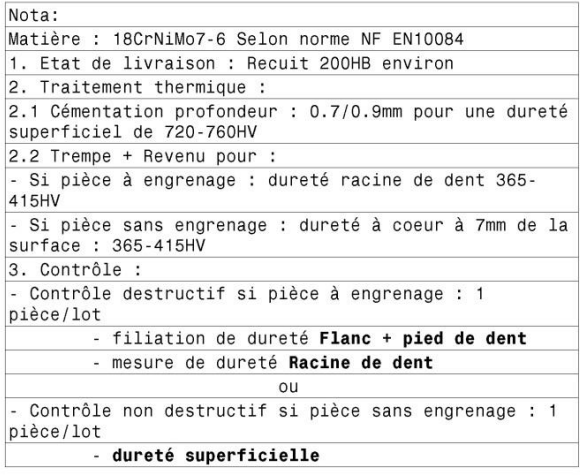
\includegraphics[width=\linewidth]{fig_02}
%\textit{}
\end{center}

Le banc d'essai est composé d'un tube représentant le corps du réacteur et d'une tuyère à ouverture variable
actionnée par quatre vérins hydrauliques et permettant de faire varier la vitesse de l'air éjecté. 

%\begin{center}
%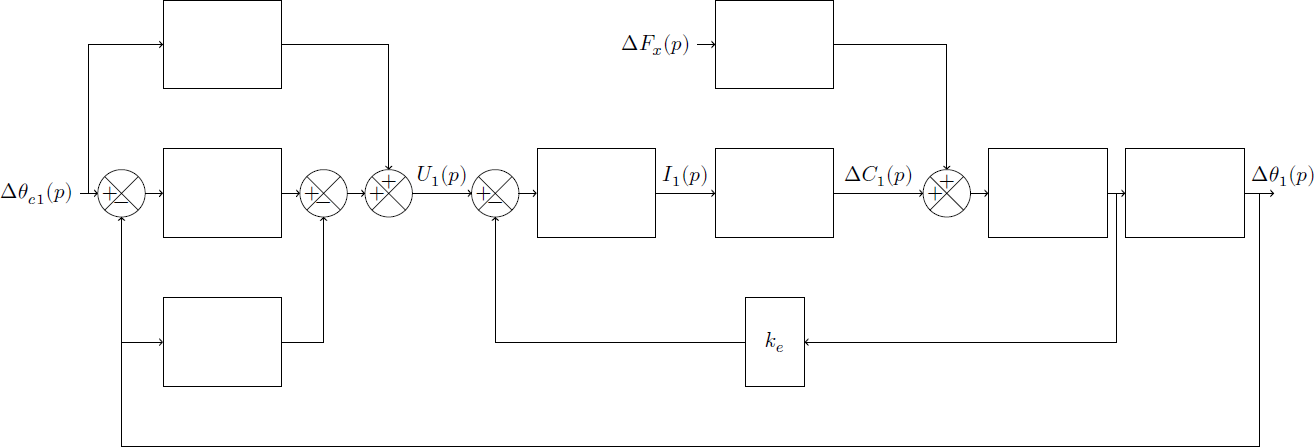
\includegraphics[width=.8\linewidth]{fig_03}
%%\textit{}
%\end{center}

\begin{center}
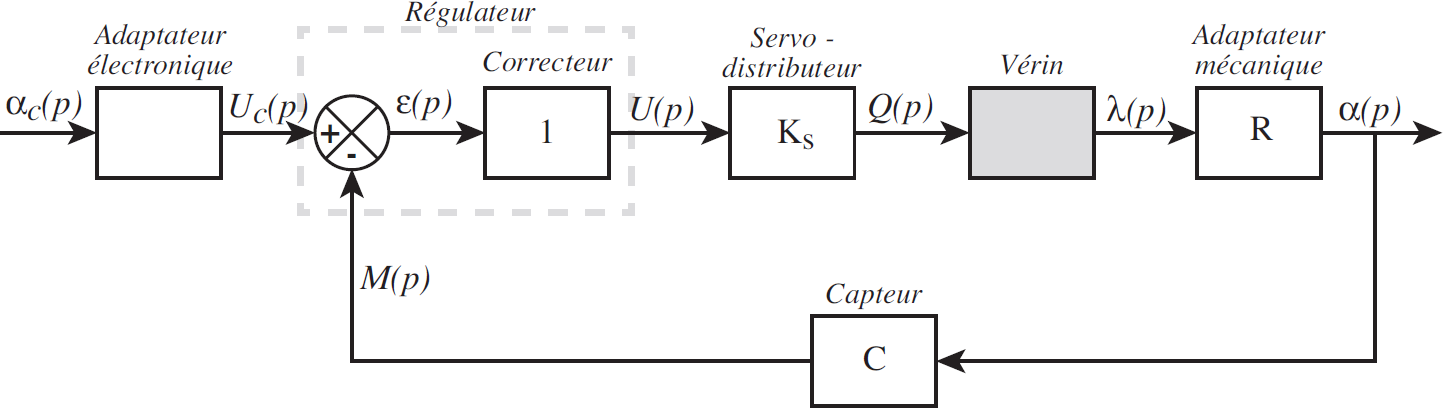
\includegraphics[width=.8\linewidth]{fig_04}
%\textit{}
\end{center}

\fi

\begin{obj}
On souhaite vérifier que le système permet de respecter le cahier des charges suivant : 
\begin{itemize}
\item temps de réponse à 5\% : \SI{4}{s} au maximum;
\item précision : l'erreur statique doit être nulle;
\item précision : l'erreur de traînage doit être inférieure à \SI{1}{mm} pour une consigne de \SI{25}{mm.s^{-1}}.
\end{itemize}
\end{obj}


\subsection*{Modélisation du comportement du vérin -- hypothèse fluide compressible}
\ifprof
\else

\begin{obj}
Il s'agit ici de proposer un modèle plus affiné du comportement du vérin en tenant compte de la compressibilité du fluide et du comportement dynamique du mécanisme.
\end{obj}		



Pour rendre compte du comportement dynamique du système on propose un modèle de comportement du vérin en tenant compte de la compressibilité du fluide. L'évolution du débit est alors une fonction du déplacement mais aussi de la pression sous la forme de la relation suivante : $q(t)=S\dfrac{\dd x(t)}{\dd t}+\dfrac{V_0}{B}\dfrac{\dd \sigma(t)}{\dd t}$ avec : 
\begin{itemize}
\item $\sigma(t)$ : pression utile dans le vérin. On notera $\Sigma(p)$ sa transformée;
\item $V_0$ : demi volume de fluide contenu dans le vérin;
\item $B$ : coefficient de compressibilité du fluide.
\end{itemize}  

La pression utile induit l'effort développé par le vérin que nous noterons $F_v$ tel que : $F_V(p)=S\Sigma(p)$ où $S$ représente la section utile du vérin en sortie de tige.

$V(p)$ représente l'image par la transformation de Laplace de la vitesse de translation $v(t)$ de la tige du vérin. 

En considérant les actions de pesanteur négligeables et en se plaçant dans une phase de test à vide (sans flux d'air), l'application des lois de la dynamique donne la relation suivante : $F_V(t)=M_{\text{eq}} \dfrac{\dd^2 x(t)}{\dd t^2}$.

\fi 

\question{À partir des équations, compléter le schéma-blocs en indiquant les fonctions de transferts de chaque bloc.}
\ifprof
\begin{corrige} ~\\
\begin{center}
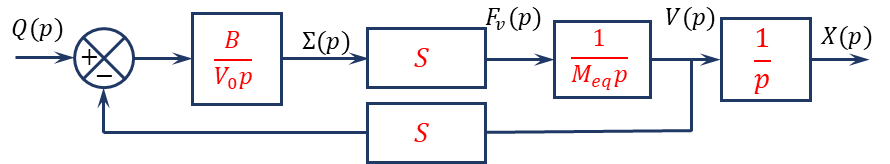
\includegraphics[width=.95\linewidth]{cor_01_b}
%\textit{}
\end{center}

\end{corrige}
\else
\
\begin{center}
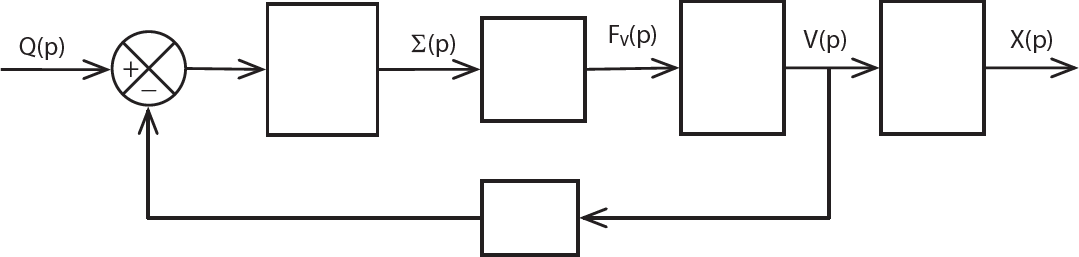
\includegraphics[width=\linewidth]{fig_05}
%\textit{}
\end{center}

On note $F_R$ l'action mécanique résistante équivalente pour quatre volets. On a $F_R(t) = K_F x(t)$. L'application du théorème de l'énergie cinétique se traduit par $M_{\text{eq}}\ddot{x}(t)=\left(F_V(t)-F_R(t)\right)$. 
\fi

\question{Modifier le schéma-blocs précédent pour intégrer l'effort résistant.}
\ifprof
\begin{corrige} ~\\
\begin{center}
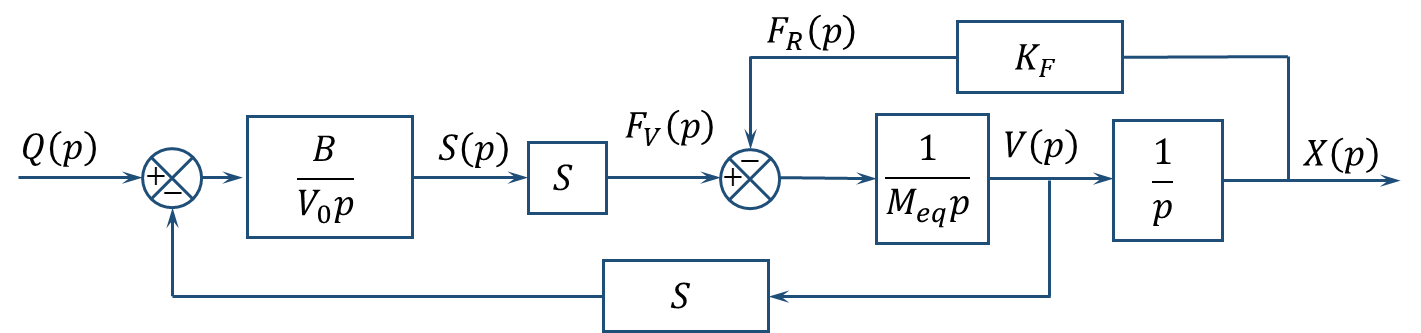
\includegraphics[width=.95\linewidth]{cor_02_b}
\end{center}
\end{corrige}
\else
\fi

\question{Donner l'expression de la fonction de transfert du vérin $H_V(p)=\dfrac{X(p)}{Q(p)}$. On donnera le résultat sous la forme $H_V(p)=\dfrac{K_V}{p\left(1+a_2 p^2 \right)}$ en précisant les expression de $K_V$ et $a_2$.}
\ifprof
\begin{corrige} ~\\
\begin{center}
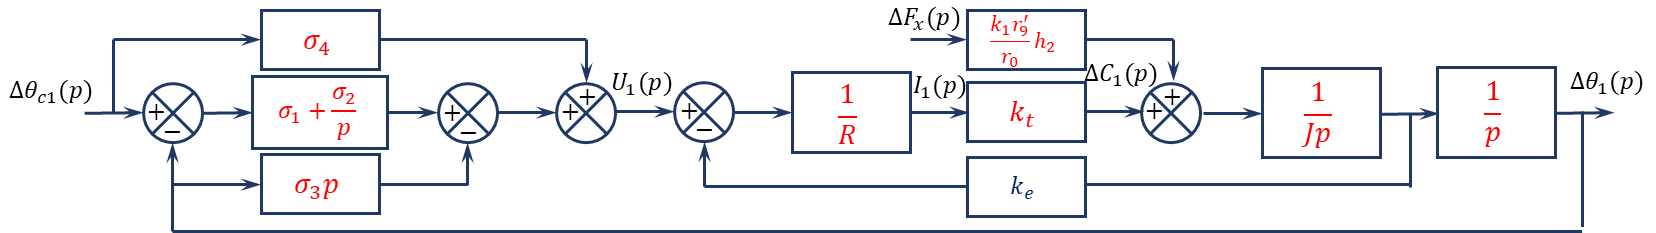
\includegraphics[width=\linewidth]{cor_03}
\end{center}
\end{corrige}
\else
\fi

\subsection*{Validation du comportement du vérin} 

\ifprof
\else

Afin de valider le modèle établi, on se propose d'étudier le comportement en boucle fermée de la chaîne fonctionnelle de commande du vérin. On rappelle ci-dessous le schéma-bloc retenu et on considérera une correction proportionnelle telle que  $C(p)=K_p$.

\begin{center}
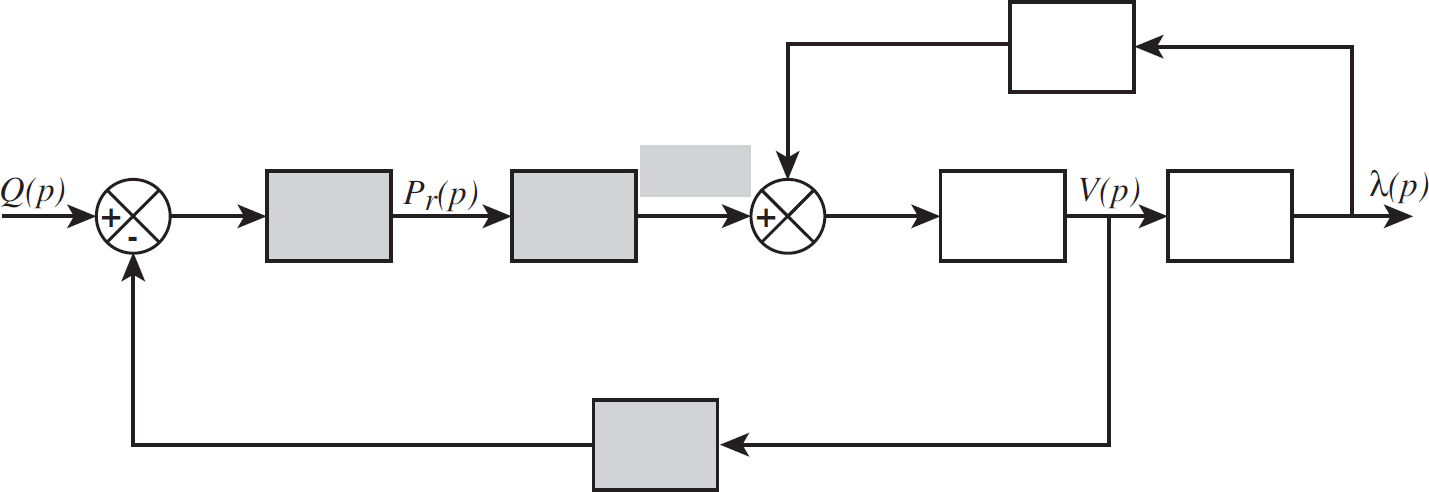
\includegraphics[width=\linewidth]{fig_06}
%\textit{}
\end{center}
\fi

\question{Donner  l'expression de la forme canonique de la fonction de transfert en boucle fermée $H_{\text{BF}}(p)=\dfrac{X(p)}{X_{\text{ref}}(p)}$ . On donnera le résultat en fonction de $K_C$, $K_U$, $K_D$, $K_p$, $K_V$ et $a_2$. }
\ifprof
\begin{corrige} ~\\
\begin{center}
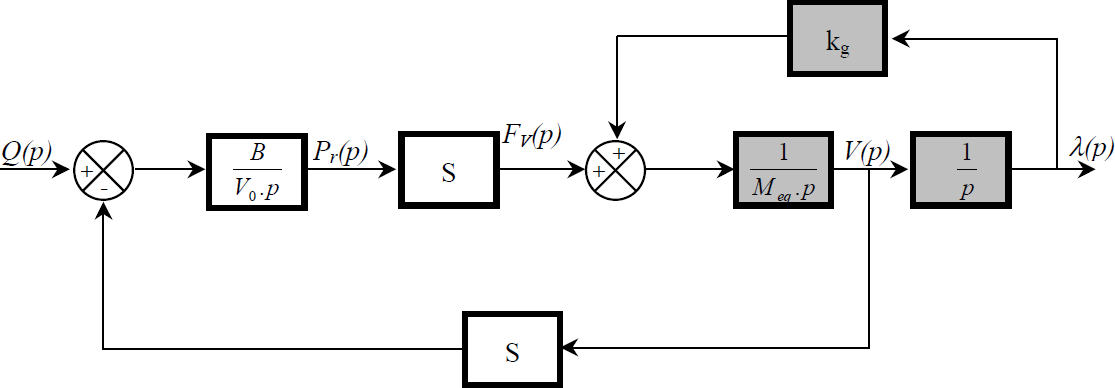
\includegraphics[width=\linewidth]{cor_04}
\end{center}
\end{corrige}
\else
\fi

\subsection*{Prise en compte du débit de fuite} 
\ifprof
\else

Pour pallier le problème de stabilité du modèle précédemment établi, une solution possible consiste à un introduire un débit de fuite entre les deux chambres du vérin. Celui-ci a pour effet de réduire artificiellement le débit réel entrant dans le vérin en fonction de la pression utile. Ce débit vaut alors : $q(t)-\delta \sigma (t)$  où $\delta$ est le coefficient de débit de fuite.
\fi

\ifprof
\newpage
\else \fi

\question{Modifier le schéma-blocs précédent pour intégrer le débit de fuite.}
\ifprof
\begin{corrige} ~\\
\begin{center}
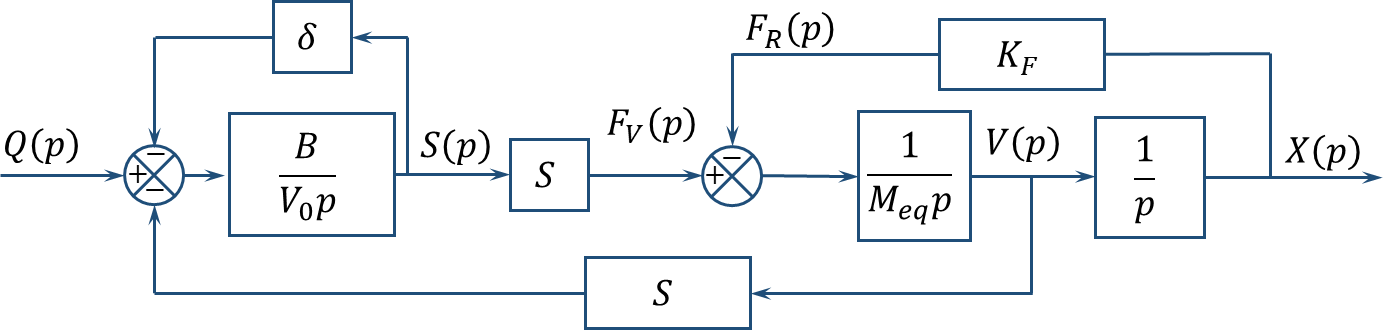
\includegraphics[width=.95\linewidth]{cor_03_b}
\end{center}
\end{corrige}
\else
\fi


\question{Donner l'expression de la fonction de transfert du vérin $H_V(p)=\dfrac{X(p)}{Q(p)}$. On donnera le résultat sous la forme $H_V(p)=\dfrac{K_V}{p\left(1+a_1 p + a_2 p^2+ a_3 p^3 \right)}$ en précisant les expression de $K_V$, $a_1$, $a_2$ et $a_3$.}
\ifprof
\begin{corrige} ~\\
\begin{center}
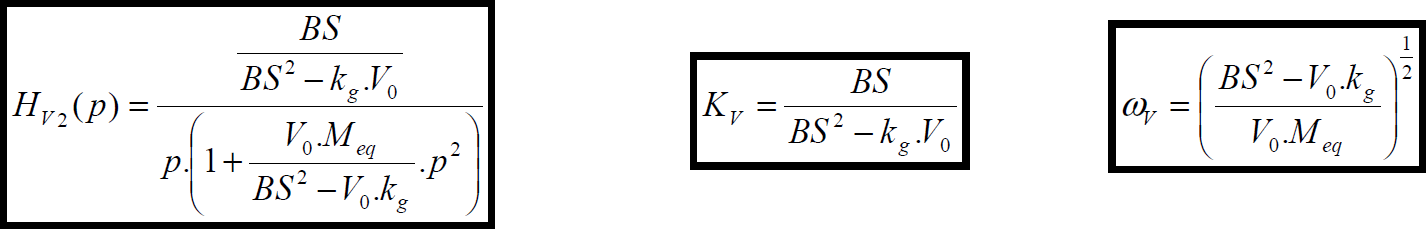
\includegraphics[width=.95\linewidth]{cor_06}
\end{center}
\end{corrige}
\else
\fi
\subsection*{Retour sur le cahier des charges}
On donne la réponse à un échelon et à une rampe de pente \SI{25}{mm.s^{-1}}.

\question{Le cahier des charges est-il vérifié ?}


\begin{center}
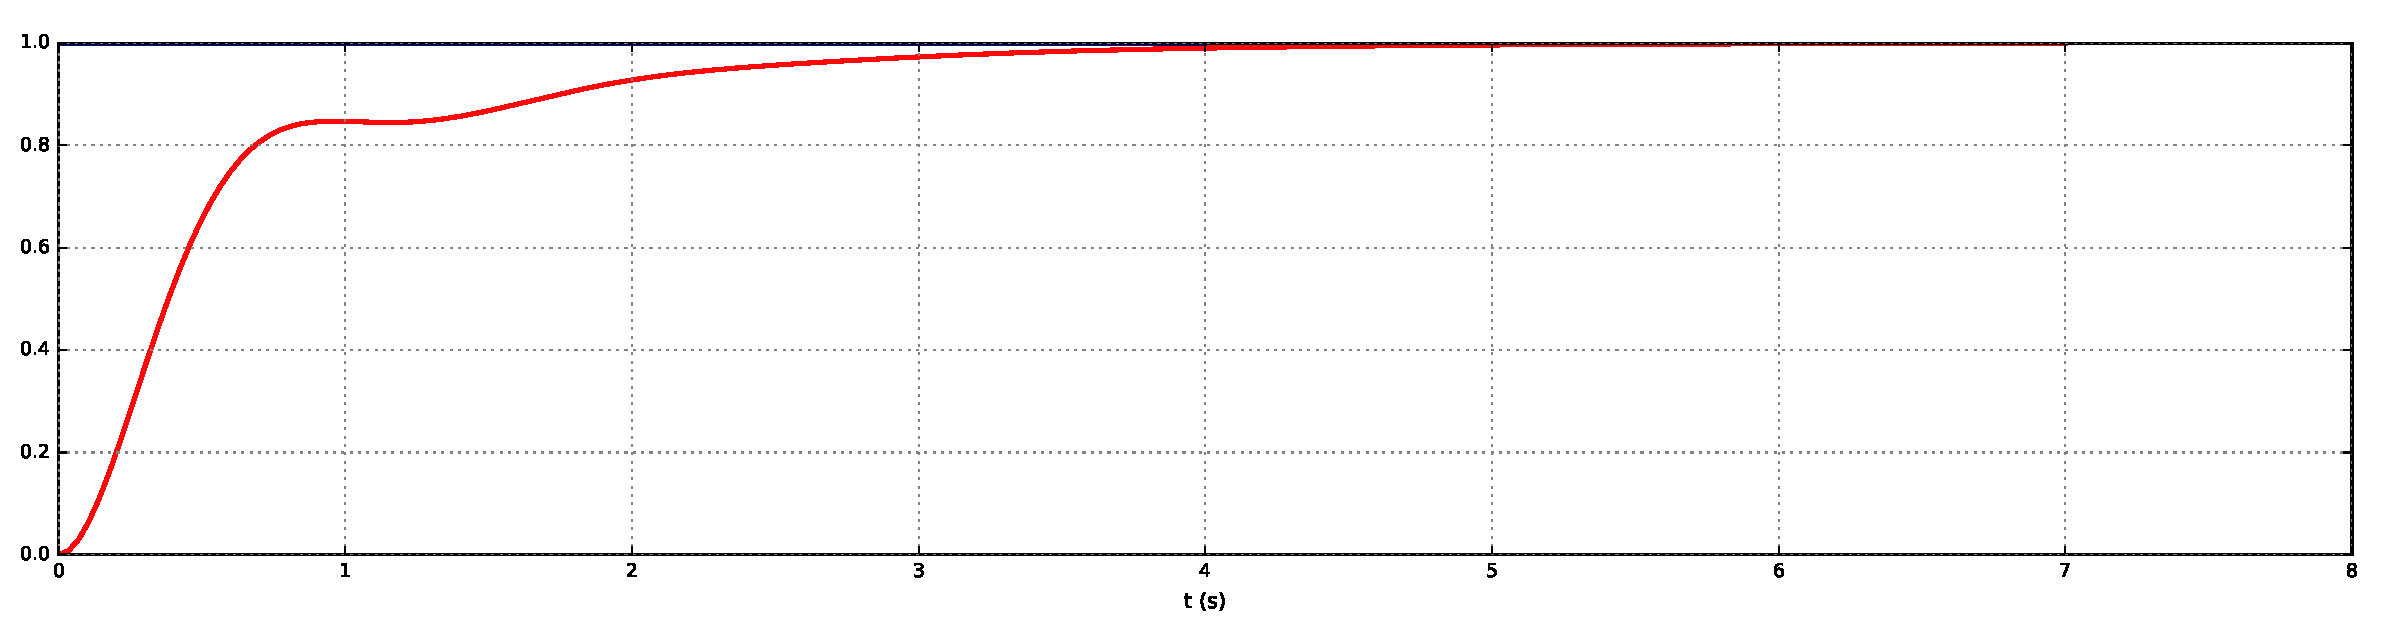
\includegraphics[width=\linewidth]{echelon}
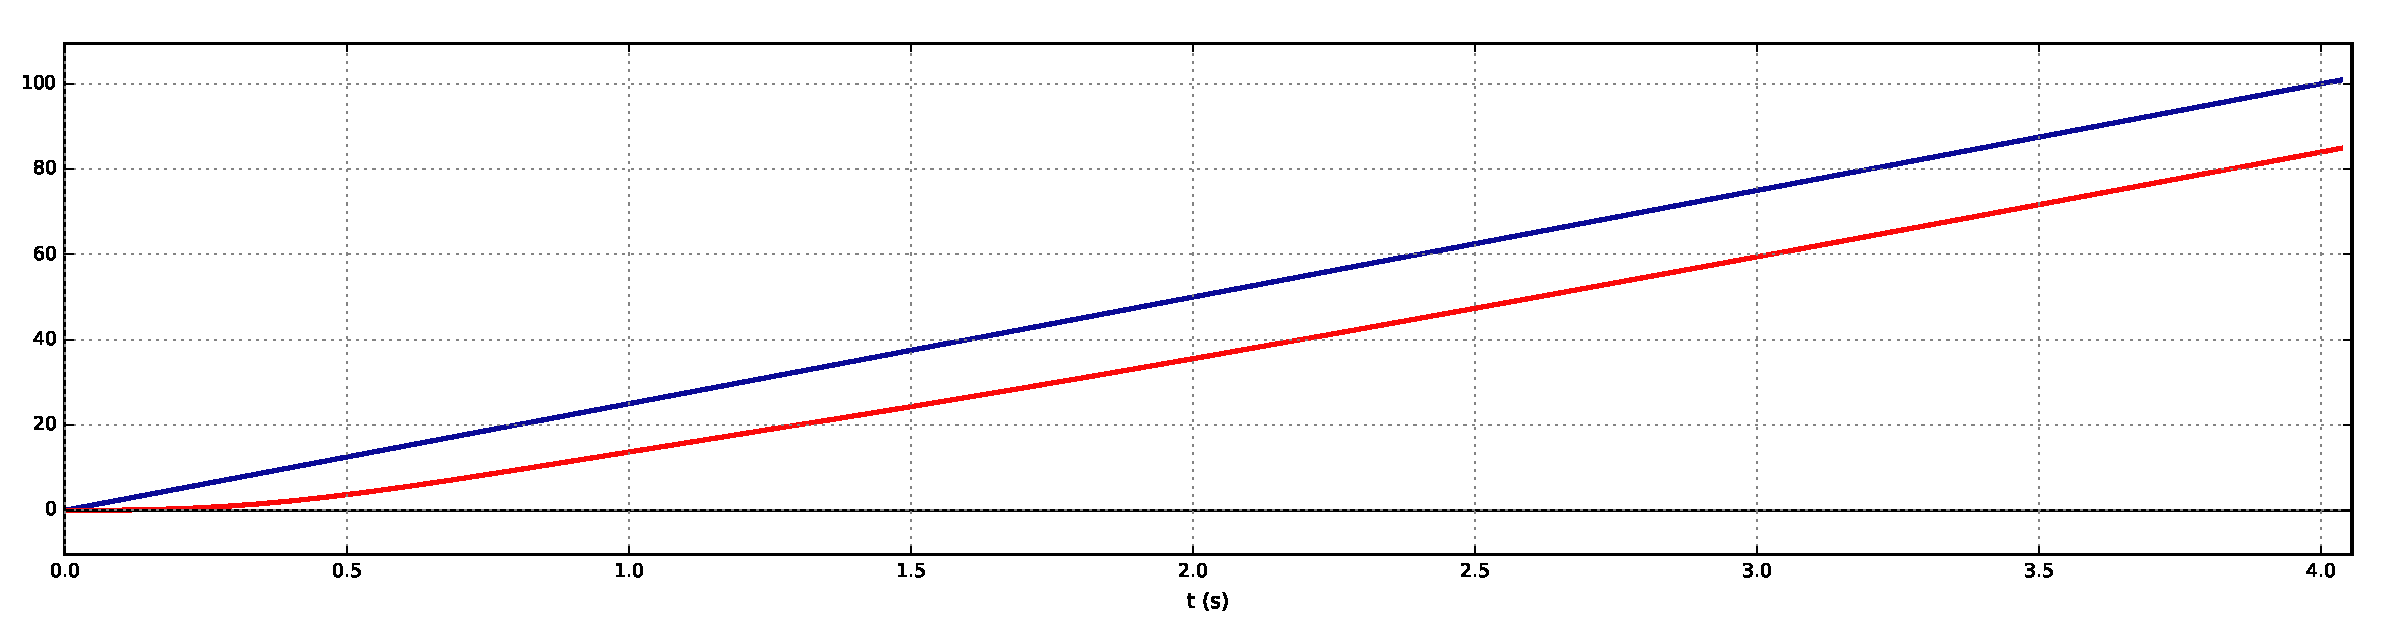
\includegraphics[width=\linewidth]{rampe}
%\textit{}
\end{center}




\ifprof
\else
\begin{flushright}
\footnotesize{Corrigé  voir \ref{B2:07:79}.}
\end{flushright}%
\fi